

%\chapter{Modeling the noise transmission}

\subsection*{II. Ornstein-Uhlenbeck fluctuations model}

\subsubsection*{Introduction}

In these notes I discuss a model which models how noise originates and transmits from and between observables respectively. I will discuss the model proposed by Philippe Nghe in the work by Kiviet et al. \cite{Kiviet2014}, and also possible extensions and modifications to this model.

Parameters that are considered in general are the number of enzymes ($E$), the rate at which these enzymes are made ($p$), and the growth rate of the cell ($\lambda$). Generally, enzymes only disappear by dilution due to growth. Furthermore, there are noise sources, which add noise to these parameters. Depending on how they are implemented these source appear as $N_M$, $N_\lambda$ and $N_p$ or $\Gamma_M$, $\Gamma_\lambda$ and $\Gamma_p$, the subscripts indicate to which parameter the noise source adds noise.

The goal of this model is to interpret the cross-correlations between $\lambda$, $E$ and $p$ (usually $R_{E,\lambda}(\tau)$, $R_{p,\lambda}(\tau)$), that are obtained from experimental data.

\subsubsection*{Implicit noise equations}


\begin{figure}
	\centering
	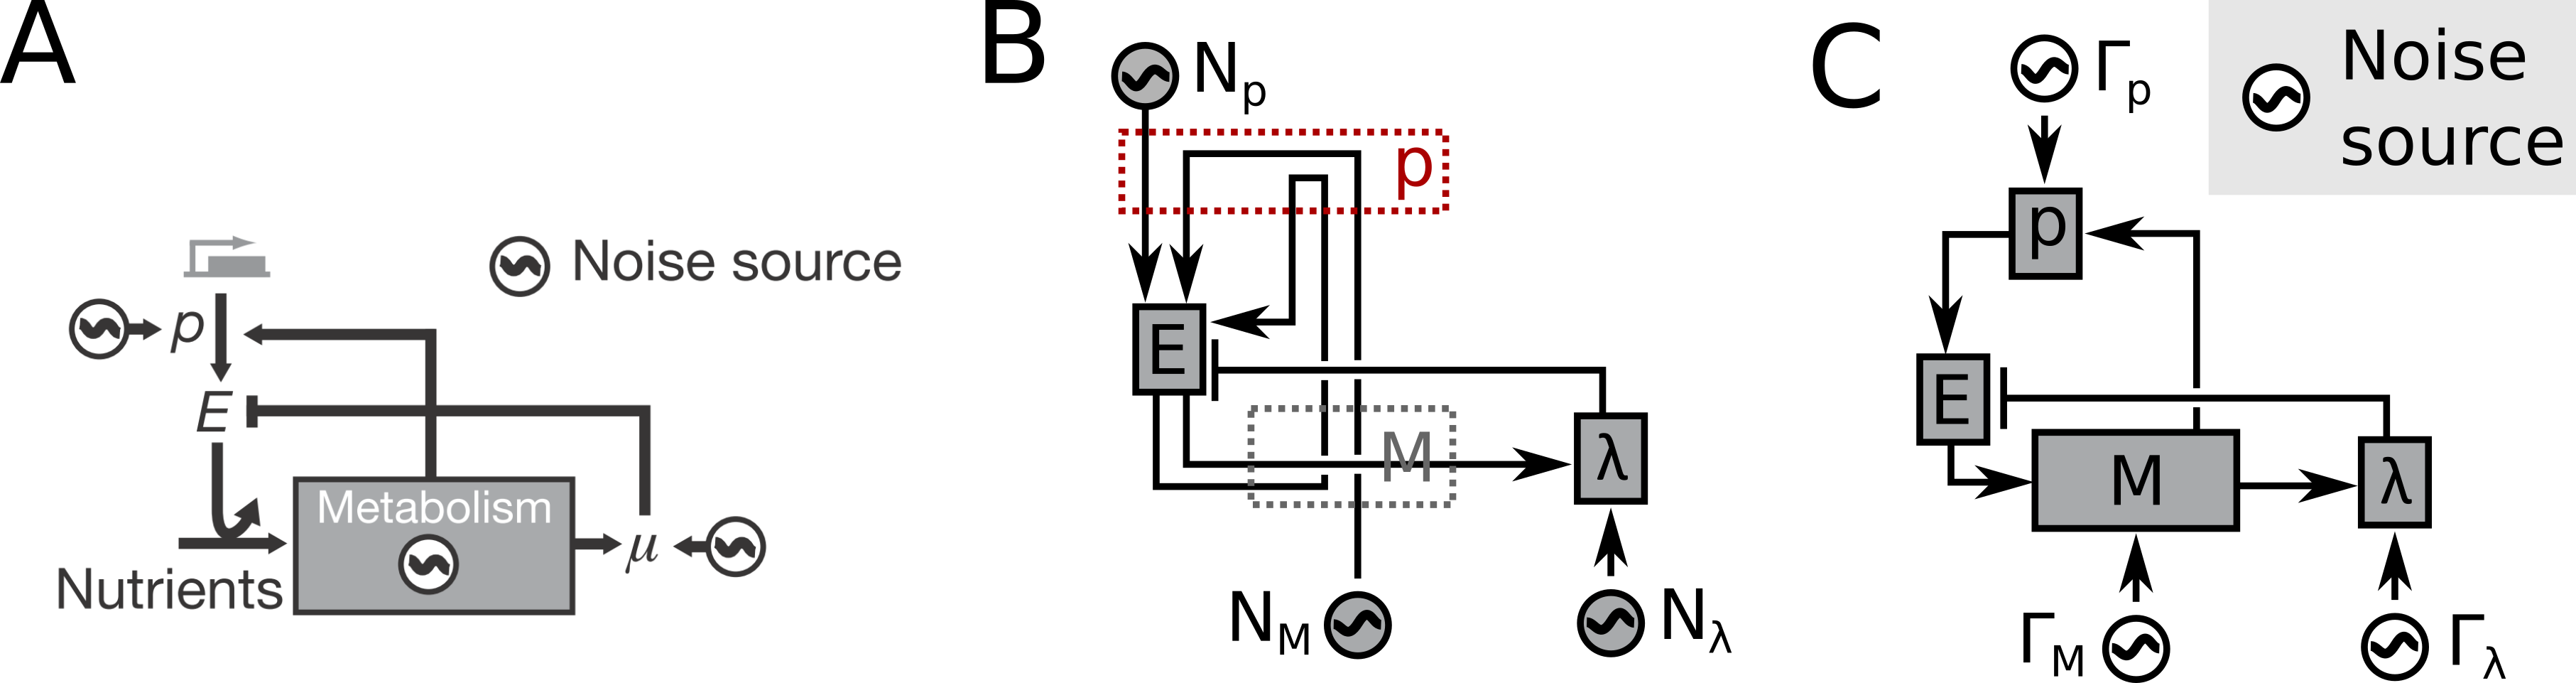
\includegraphics[width=0.9\textwidth]{model_nghe_v2.png}
	\caption{ 
		(A) Original diagram as printed in Kiviet et al. \cite{Kiviet2014}.
		(B) More technical diagram stating the relations between parameters of interest (gray boxes), and noise sources $N_P$, $N_M$, and $N_\lambda$. Arrows indicate how ODEs or functions that describe the parameters of interest are coupled. 
		Arrows that go trough the red dashed box correspond to terms that not only couple the two parameters connected by the arrow, but also make up the parameter $p$ (see also main text).
		Arrows that go through the grey box are arrows which are thought to be biologically connected to the metabolism.
		(C) An alternative version of the model with more parameters modelled explicitly. Noise sources are printed white in this diagram since they are not described by separate ODEs, which was the case in Kiviet et al. \cite{Kiviet2014}. 
	}
	\label{fig:modeldrawing}
\end{figure}

A straight forward way to model a system with these parameters, is writing down an ordinary differential equation (ODE) for each parameter involved. 
%
The Nghe model takes a somewhat different approach (it is more concise), which will be discussed later.
%
The ODEs below relate to the cartoon in Fig. \ref{fig:modeldrawing}.C
and describe the dynamics per parameter:
%
\begin{align}
\label{myfirstequation}
\dot{M} = & - \frac{(M-M_0)}{\tau}  \nonumber \\ 
          & + c_M \cdot \Gamma_M  \nonumber \\ % (1-T_{M\leftarrow E})
          & + T_{M\leftarrow E} \cdot c_M' \cdot (\frac{E}{E_0} - 1)  
\end{align}
% deltaMetabolism = -(metabolismValues(end)-parameters.metabolism0) * 1/parameters.dampingTimeMetabolism + ... % damping; 1 is the equilibrium value
% (1-parameters.transmissionEnzymeMetabolism) * ((rand()-.5)*2) * parameters.noiseSizeMetabolism + ...                              % white noise component
% parameters.transmissionEnzymeMetabolism * (enzymeValues(end)/parameters.enzymeTarget-.5) * parameters.noiseSizeMetabolism;             % noise component due enzyme
%
%
\begin{align}
	\dot{\lambda} = & -\frac{(\lambda - \lambda_0 )}{\tau_\lambda} \nonumber \\ 
 			& + c_\lambda \cdot \Gamma_\lambda \nonumber \\  %  (1-T_{\lambda\leftarrow M}) \cdot
			& + T_{\lambda\leftarrow\ M} \cdot c_\lambda' \cdot (\frac{M}{M_0}-1) 
\end{align}
%
\begin{align}
\label{mythirdequation}
\dot{P} = & - \frac{(P-P_0)}{\tau_P} \nonumber \\ 
		 & + c_p \cdot \Gamma_p \nonumber \\ 
         & + T_{P\leftarrow M} \cdot c_P' \cdot (\frac{M}{M_0}-1)  \nonumber \\ 
         & + R_{P\leftarrow M} \cdot c_P' \cdot (\frac{M}{M_0}-1)
\end{align}
%
\begin{align}
\label{mylastequation}
\dot{E} = P - \lambda E
\end{align}
%
Where $M$ describes the state of the metabolism, $\lambda$ is the growth rate, $P$ is the production rate, $E$ is the amount of enzyme, $\tau$ is a dampening term ($X_0$ is the equilibrium value), $T_{X \leftarrow Y}$ is the noise transmission constant from $X$ towards $Y$, $c_X$ and $c_X'$ are constants that set the size of the fluctuations, $\Gamma_X$ is a white noise source.
$R_{X \leftarrow Y}$ indicates a regulatory interaction, an addition to the model, but this notation is just cosmetic, as $T_\text{effective}=T+R$.
%
This model assumes all parameters have an average value from which fluctuations deviate, but always return. Hence the dampening terms.
With respect to transmission, I furthermore rescale the absolute value of the noise to be comparable to the target noise (hence the $M_0^{-1}$ and $c_X$ terms in combination with the $T_{X\leftarrow Y}$ term).

This is similar to the model that Philipe Nghe suggested in Kiviet et al. \cite{Kiviet2014}, which was inspired by Dunlop et al. \cite{Dunlop2008} (see supplement of that manuscript for a description of the Dunlop model).
%
A difference between my equations, the Nghe equations and the Dunlop equations lies in the dampening terms (those containing $\tau$, $\beta$ or $\mu_E$). In my model noise is effected through the ODE, and dampening occurs on the parameter of interest. In Dunlop et al., there are two dampening terms, one specifically dampening the noise and a second term dampening the parameters of interest. \red{Nghe also takes the latter approach, see below.}
% dampening being effected through the $(-\beta_X \cdot N_X)$ term and the $\mu_E$ parameter (see later for a more involved discussion on these parameters)}.

The correlations between these equations can be found by linearizing them, writing the correlations in Fourier space, and back-transforming them using residue integration techniques. 
\red{These notes do} not fully explores this, but \red{this will partially be discussed later}.
First, a comparison of the above model with the Nghe model is made.

\subsubsection*{Numerical implementation}

Out of practical considerations, we numerically solved Eq. \ref{myfirstequation}-\ref{mylastequation} by simple Euler propagation implemented in Matlab.
%
The script \texttt{growthnoisepropagatorv2.m} will be made available in an online Github repository, parameter settings that were used are shown below.
%
For the dilution mode: 
\begin{gather*}
E_0= 2000,
\mu_0= 1,
%\lambda_0= 0.6931,
\lambda_0= 0.0116, 
\nonumber \\ p_0= 23.1049, 
C_0= 1,
\tau_\lambda= 120,
\Gamma_\lambda= 8.3255e-04,
\Gamma_\lambda'= 8.3255e-04,
\nonumber \\ \tau_p= 120,
\Gamma_p= 0.0048,
\Gamma_p'= 0.0048,
\tau_C= 120,
\Gamma_C= 1.0000e-03,
\Gamma_C'= 1.0000e-03,
%dampingNoiseOnly= Inf,
\nonumber \\ T_{C\rightarrow\lambda}= 0,
T_{C\rightarrow{p}}= 0,
T_{E\rightarrow{C}}= 1,
T_{\lambda\rightarrow{E}}= -1;
%interactionCProduction= 0,
\end{gather*}
%
($\lambda$ is given in units of $min^{-1}$ here.)
For the catabolic mode: 
\begin{gather*}
E_0= 2000,
\mu_0= 1,
%\lambda_0= 0.6931,
\lambda_0= 0.0116,
\nonumber \\ p_0= 23.1049,
C_0= 1,
\tau_\lambda= 60,
\Gamma_\lambda= 0,
\Gamma_\lambda'= 8.3255e-06,
\nonumber \\ \tau_p= 60,
\Gamma_p= 1.5200,
\Gamma_p'= 1.5200,
\tau_C= 60,
\Gamma_C= 0,
\Gamma_C'= 0.3162,
%dampingNoiseOnly= Inf,
\nonumber \\ T_{C\rightarrow\lambda}= 0.9000,
T_{C\rightarrow{p}}= 0,
T_{E\rightarrow{C}}= 0.9000,
T_{\lambda\rightarrow{E}}= -1;
%interactionCProduction= 0,
\end{gather*}
For the common mode: 
\begin{gather*}
E_0= 2000,
\mu_0= 1,
%\lambda_0= 0.6931,
\lambda_0= 0.0116,
\nonumber \\p_0= 23.1049,
C_0= 1,
\tau_\lambda= 6,
\Gamma_\lambda= 0,
\Gamma_\lambda'= 8.3255e-06,
\nonumber \\ \tau_p= 6,
\Gamma_p= 0,
\Gamma_p'= 0.0481,
\tau_C= 60,
\Gamma_C= 0.3162,
\Gamma_C'= 0.3162,
%dampingNoiseOnly= Inf,
\nonumber \\ T_{C\rightarrow\lambda}= 0.9000,
T_{C\rightarrow{p}}= 0.9000,
T_{E\rightarrow{C}}= 0,
T_{\lambda\rightarrow{E}}= -1;
%interactionCProduction= 0,
\end{gather*}
For the combined scenario: 
\begin{gather*}
E_0= 2000,
\mu_0= 1,
%\lambda_0= 0.6931,
\lambda_0= 0.0116,
\nonumber \\p_0= 23.1049,
C_0= 1,
\tau_\lambda= 60,
\Gamma_\lambda= 2.4034e-04,
\Gamma_\lambda'= 2.4034e-04,
\nonumber \\ \tau_p= 60,
\Gamma_p= 0.5308,
\Gamma_p'= 0.5308,
\tau_C= 60,
\Gamma_C= 0.1459,
\Gamma_C'= 0.1459,
%dampingNoiseOnly= Inf,
\nonumber \\ T_{C\rightarrow\lambda}= 0.2700,
T_{C\rightarrow{p}}= 0.3000,
T_{E\rightarrow{C}}= 0.2700,
T_{\lambda\rightarrow{E}}= -1,
%interactionCProduction= -0.2700,
\end{gather*}
%
Cross-correlations were calculated based on 100000 one-minute timesteps, noise was introduced with the matlab function \texttt{normrnd}.
% 
The feedback is added by subtracting $0.27$ from the $T_{C\rightarrow\lambda}$ parameter, i.e. setting it to zero.

\subsection*{Separate noise equations}

Both Nghe and Dunlop define separate ODEs for the noise terms:
%
\begin{align}
\label{eq:generalgillespienoise}
\dot{N}_X = \sqrt{C_X} \cdot \Gamma_X - N_X/\tau
,
\end{align}
%
though their notation might be slightly different (I used Daniel Gillespie's notation \cite{Gillespie1996}; a capital C is used here to follow Gillespie's square root notation, $\sqrt{C_X}=c_x$).
With for our case $X$ equaling $\lambda$, $M$ or $P$. Note that $\tau^{-1}=\beta$ ($\beta$ is used in Nghe and Dunlop).

Not so relevant for our case, but noteworthy, is that in the Dunlop model, which models a completely different process than the one described here \cite{Dunlop2008}, the \textit{solutions} of the ODEs describing the noise are plugged into the ODEs describing the protein dynamics. This leads to an additional memory effect.
%
That is:
%
\begin{align}
\label{dunlopgeneralequation}
\dot{X} = & N_X  + F(X) + X/\tau
,
\end{align}
%
with $F(X)$ some arbitrary function of $X$. 
Note that the $N_X$ function also contains a $\tau$ term (see Eq. \ref{eq:generalgillespienoise}), which is effectively integrated, thus leading to effects of the fluctuations much longer timescales than $\tau$. 
This effect is (partially) countered by the third term in Eq. \ref{dunlopgeneralequation}, which also contains the $\tau$ term.

\subsection*{Nghe model}

As mentioned, the Nghe model takes a different approach. 
The formulae that follow correspond to Fig. \ref{fig:modeldrawing}.B (Fig. \ref{fig:modeldrawing}.A contains the version of the cartoon which was published in Kiviet et al.).
The starting point,
%
\begin{align}
\label{eq:Nghe1}
\dot{E} = P - \lambda E
,
\end{align}
%
is the same in my model, but after linearization (defined as $X=X_0+\delta X$) this leads to only one ODE:
% CONVENIENT NOTE TO SELF: %%%%%%%%%%%%%%%%%%%%%%%%%%%%%%%%%%%%%%%%%%%
% See written notes from 28.9.2016 for explicit linearization.
% END CONVENIENT NOTE TO SELF: %%%%%%%%%%%%%%%%%%%%%%%%%%%%%%%%%%%%%%%
%
\begin{align}
\label{eq:ODEElinearized}
\frac{ \delta{\dot{E}} }{E_0 \mu_0} 
+ \frac{\delta E}{E_0} 
%& = 
%\left[
% T_{E \leftarrow E} \frac{\delta E}{E_0} + T_{E \leftarrow G} N_G + N_E 
% \right]
% + T_{E \leftarrow \mu} \frac{\delta \mu}{\mu_0} \nonumber \\
& =
\frac{\delta p}{E_0 \mu_0} + T_{E \leftarrow \mu} \frac{\delta \mu}{\mu_0}
.
\end{align}
%
Noise terms are introduced with ODEs that are also shown above in Eq. \ref{eq:generalgillespienoise}.
 Additionally, two functions are defined for $p$ and $\lambda$. These are not ODEs, as the effects on these parameters are thought to happen on fast timescales. The parameters are however linearized (and thus written as $\delta X$). The equation
%
\begin{align}
\label{eq:Nghe3}
\frac{\delta\mu}{\mu_0} = T_{\mu \leftarrow E} \frac{\delta E}{E_0} + T_{\mu \leftarrow G} N_G + N_\mu
\end{align}
%
simply defines the evolution of $\delta \mu$.
There is also a similar equation for $\delta p$:
%
\begin{align}
\label{eq:Nghe4}
\frac{\delta{p}}{E_0 \mu_0} = T_{E \leftarrow E} \frac{\delta E}{E_0} + T_{E \leftarrow G} N_G + N_E
,
\end{align}
%
which plays a bit more complicated role.
It is defined using terms that pertain to E, like $T_{E \leftarrow G}$, such that it can be directly plugged into Eq. \ref{eq:ODEElinearized}. 
Indeed, plugging Eq. \ref{eq:Nghe4} into Eq. \ref{eq:ODEElinearized} leads to equation:
%
\begin{align}
\label{eq:Nghe5}
\frac{ \delta{\dot{E}} }{E_0 \mu_0} 
+ \frac{\delta E}{E_0} 
& = 
\left[
 T_{E \leftarrow E} \frac{\delta E}{E_0} + T_{E \leftarrow G} N_G + N_E 
 \right]
 + T_{E \leftarrow \mu} \frac{\delta \mu}{\mu_0} 
\end{align}
%
which corresponds to equation 5 in the Kiviet et al. \cite{Kiviet2014} manuscript.
I say it is a bit complicated, since Eq. \ref{eq:Nghe4} has no role in the model (we could also just have defined Eq. \ref{eq:Nghe5} immediately), except that it shows us which part of the model can be interpreted as being the production rate.
This is also the reason why $p$ is depicted as a red dashed box in Fig. \ref{fig:modeldrawing}.

%
%{\color{red}
%There are currently a few things unclear about Eq. \ref{eq:Nghe3} and Eq. \ref{eq:Nghe4} (respectively Eq. 3 and 4 in the Kiviet et al. manuscript):
%\begin{itemize}
%\item It seems that the transmission terms $T_{X\leftarrow Y}$ state how the parameter of interest ($X$) is affected by another parameter of interest ($Y$), however, for this to be true, the left-hand side parameter should match the first parameter in the subscript of $T$. E.g. how can a $T_{E\leftarrow G}$ term appear in the equation for $\delta p$ and moreover, what does the term $T_{E \leftarrow E}$ mean?
%\item It is not clear to me how these formulae relate to the diagram that was drawn (see Fig. \ref{fig:modeldrawing}). Why is E directly effecting $\mu$? Should there not also be a metabolism term $G$ or $\delta G$? Also why does the formula for $\delta p$ contain transmission from $E$ (assuming $T_{E\leftarrow E}$ was a type and should have been $T_{p\leftarrow E}$)? Why does the formula for $\delta p$ contain a noise term for E (ie. $N_E$)?
%\item These are not ODEs (which would seem more natural to me), probably this is intended this way, and the relationship between the parameters is defined as such. (And could be derived from ODEs.)    
%\end{itemize}
%%I am currently not sure how these equations relate to my own equations, as subscripts in Eq. \ref{eq:Nghe4} seem inconsistent with the fact that transmission should be towards $P$ (e.g. what is $T_{E\leftarrow E}$?).
%}
%
%In any case, given that noise and other parameters are related in terms of parameters (not derivatives), the following formulae are probably underlying the Nghe model:
%
%\begin{align}
%\dot{M} = & \dot{N}_M  \nonumber \\ 
%& + T_{M\leftarrow E} \cdot c_M \cdot (\frac{E}{E_0} - 1)  
%\end{align}
%
%\begin{align}
%\dot{\lambda} = & \dot{N}_\lambda \nonumber \\ 
%& +    T_{\lambda \leftarrow M} \cdot c_\lambda \cdot (\frac{M}{M_0}-1) 
%\end{align}
%
%\begin{align}
%\dot{P} = & \dot{N}_P \nonumber \\ 
%& + T_{P\leftarrow M} \cdot c_P \cdot (\frac{M}{M_0}-1)  \nonumber \\ 
%& + R_{P\leftarrow M} \cdot c_P \cdot (\frac{M}{M_0}-1)
%\end{align}
%
%Where the normalizations by $X_0$ were left out again.

Note that dampening terms can be implicitly present in the Nghe model, in the form of a transmission from the parameter to itself.
Specifically, $T_{E \leftarrow E}$ can fulfill this role. % when it is negative and $<1$. 
Second order dampening can also occur, 
as is pointed out in the Kiviet et al supplementary information, which states that the time scale of the $E$ fluctuations is set by the term $\mu_0(1-T_{E \leftarrow \mu}T_{\mu \leftarrow E}-T_{E \leftarrow E})$.

% I previously thought that dampening was not present in the Nghe model, but this is not the case.
% Here the previous text:
%Note however, that this results in the absence of dampening terms on the parameters $X$ themselves, which might lead to 
%%non-steady state behavior of the parameters.
%unstable behavior of the parameters.
%The term $X/\tau$ could be added to each of the equations to resolve this issue; the term $-N_X/\tau$ from the noise ODEs could then be dropped.
%{\color{red}Note that a $\mu_E$ term appears eventually in Nghe's equations, which might play the role of a second dampening term.}



%%%%%%%%%%%%%%


